\chapter{Convergence en loi}
\sloppy


La loi, c'est ce qu'il y a de plus important.
\section{Définition}
Il existe des suites de variables aléatoires qui ne convergent ni presque sûrement, ni en probabilité, ni en $L^1$, mais dont la loi converge, voire est même constante.
\begin{example}
Considérons l'espace de probabilité $(\Omega, \mathcal{F}, P) = ([0,1], \mathcal{B}([0,1]), \lambda)$ où $\lambda$ est la mesure de Lebesgue.
Considérons la suite de variables aléatoires $(X_n)$ définies pour $\omega \in [0,1]$ par :
\begin{align*}
    X_{2n}(\omega) &= \mathbf{1}_{[0, 1/2]}(\omega) \\
    X_{2n+1}(\omega) &= \mathbf{1}_{[1/2, 1]}(\omega)
\end{align*}
Cette suite ne converge ni p.s., ni $L^1$, ni en probabilité, mais toutes les v.a. suivent la loi de Bernoulli de paramètre $1/2$.
\begin{figure}[H]
    \centering
    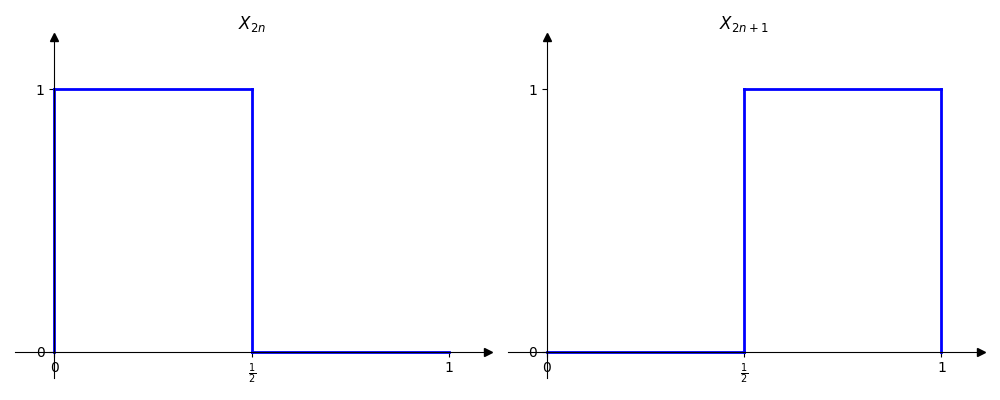
\includegraphics[width=0.6\textwidth]{convergence_en_loi_exemple.png}
    \caption{Représentation des variables aléatoires $X_{2n}$ et $X_{2n+1}$.}
    \label{fig:cv_loi_ex}
\end{figure}
Pour tout $n$, la loi de $X_n$ est la loi de Bernoulli(1/2).
\[
\forall n, P(X_n=0) = P(X_n=1) = \frac{1}{2}
\]
et donc $P_{X_n} = \text{Ber}(1/2)$ ne dépend pas de $n$.
\end{example}
\begin{definition}[Convergence en loi]
Soit $(X_n)_{n \in \mathbb{N}}$ une suite de variables aléatoires réelles (qui ne sont pas nécessairement définies sur le même espace de probabilité). La suite $(X_n)_{n \in \mathbb{N}}$ converge en loi vers une variable aléatoire $X$, ce que l'on note $X_n \xrightarrow{\mathcal{L}} X$, si et seulement si, pour toute fonction continue bornée $f: \mathbb{R} \to \mathbb{R}$,
\[
\lim_{n \to \infty} \mathbb{E}[f(X_n)] = \mathbb{E}[f(X)].
\]
\end{definition}
\begin{remark}
L'espérance $\mathbb{E}[f(X_n)]$ ne dépend que de la loi de $X_n$, i.e.,
\[
\mathbb{E}[f(X_n)] = \int_{\Omega} f(X_n) dP = \int_{\mathbb{R}} f(x) dP_{X_n}(x).
\]
Ainsi la convergence en loi s'applique même dans les situations où les v.a. $X_n$ ne sont pas définies sur le même espace de probabilité $(\Omega, \mathcal{F}, P)$, i.e. si $X_n: (\Omega_n, \mathcal{F}_n, P_n) \to (\mathbb{R}, \mathcal{B}(\mathbb{R}))$ où les $(\Omega_n, \mathcal{F}_n, P_n)$ n'ont aucun lien a priori. Ceci distingue fondamentalement la convergence en loi des autres modes de convergence.
\end{remark}
\section{La fonction de répartition}
Un outil fondamental pour étudier les lois de probabilité sur $\mathbb{R}$ est la fonction de répartition.
\begin{definition}
Soit $X$ une variable aléatoire réelle définie sur $(\Omega, \mathcal{F}, P)$. Sa fonction de répartition est la fonction $F_X$ définie par :
\[
\forall x \in \mathbb{R}, \quad F_X(x) = P(X \le x).
\]
On a $F_X(x) = P_X((-\infty, x])$. Comme les intervalles $(-\infty, x]$, $x \in \mathbb{R}$ engendrent les boréliens et forment une famille stable par intersection finie ($\pi$-système), par l'unicité du théorème d'extension de $\pi-\lambda$, la loi $P_X$ est déterminée par $F_X$.
Conclusion: la fonction de répartition $F_X$ détermine la loi $P_X$ de $X$.
\end{definition}
Une fonction de répartition $F$ vérifie:
\begin{enumerate}
    \item[i)] $F$ est croissante de $\mathbb{R}$ dans $[0, 1]$.
    \item[ii)] $F$ est continue à droite en tout point.
    \item[iii)] $\lim_{x \to -\infty} F(x) = 0$ et $\lim_{x \to +\infty} F(x) = 1$.
\end{enumerate}
\begin{proof}
\begin{enumerate}
    \item[i)] Par croissance de la mesure. Si $x_1 \le x_2$, alors $(-\infty, x_1] \subseteq (-\infty, x_2]$, donc $P(X \le x_1) \le P(X \le x_2)$.
    \item[ii)] Soit $x_0 \in \mathbb{R}$. Regardons $\lim_{x \to x_0, x > x_0} F_X(x)$.
    Soit $(x_n)_{n \in \mathbb{N}}$ une suite qui décroît vers $x_0$. Alors les ensembles $A_n = (-\infty, x_n]$ forment une suite décroissante d'événements. Par continuité monotone de la probabilité :
    \[
    \lim_{n \to \infty} F_X(x_n) = \lim_{n \to \infty} P(X \in A_n) = P(X \in \bigcap_{n=1}^\infty A_n) = P(X \in (-\infty, x_0]) = F_X(x_0).
    \]
    \item[iii)] Par continuité monotone de la probabilité. Pour la limite en $-\infty$, on prend une suite $x_n \to -\infty$ (e.g. $x_n=-n$).
    \[
    \lim_{x \to -\infty} F_X(x) = \lim_{n \to \infty} P(X \le -n) = P(\bigcap_{n=1}^\infty \{X \le -n\}) = P(\emptyset) = 0.
    \]
    Pour la limite en $+\infty$, on prend une suite $x_n \to +\infty$ (e.g. $x_n=n$).
    \[
    \lim_{x \to +\infty} F_X(x) = \lim_{n \to \infty} P(X \le n) = P(\bigcup_{n=1}^\infty \{X \le n\}) = P(X \in \mathbb{R}) = 1.
    \]
\end{enumerate}
\end{proof}
\begin{remark}
Dans certains livres, $F_X$ est définie comme $F_X(x) = P(X < x)$. Dans ce cas, la fonction de répartition est continue à gauche.
\end{remark}
\begin{example}[Fonctions de répartition de lois classiques]
\begin{enumerate}
    \item $X \sim \mathcal{B}(p)$ (loi de Bernoulli). $F_X(x) = 0$ si $x<0$, $1-p$ si $0 \le x < 1$, et $1$ si $x \ge 1$.
    \item $X \sim \mathcal{U}(\{1, \dots, n\})$ (loi uniforme discrète). $F_X(x) = \frac{\lfloor x \rfloor}{n}$ pour $1 \le x \le n$.
    \item $X \sim \mathcal{U}([0,1])$ (loi uniforme continue). $F_X(x) = 0$ si $x<0$, $x$ si $0 \le x \le 1$, et $1$ si $x>1$.
    \item $X \sim \text{Exp}(\lambda)$ (loi exponentielle). $F_X(x) = 1 - e^{-\lambda x}$ si $x \ge 0$, et $0$ si $x<0$.
    \item $X \sim \mathcal{N}(0,1)$ (loi normale centrée réduite). $F_X(x) = \int_{-\infty}^x \frac{1}{\sqrt{2\pi}} e^{-t^2/2} dt$.
\end{enumerate}
\begin{figure}[H]
    \centering
    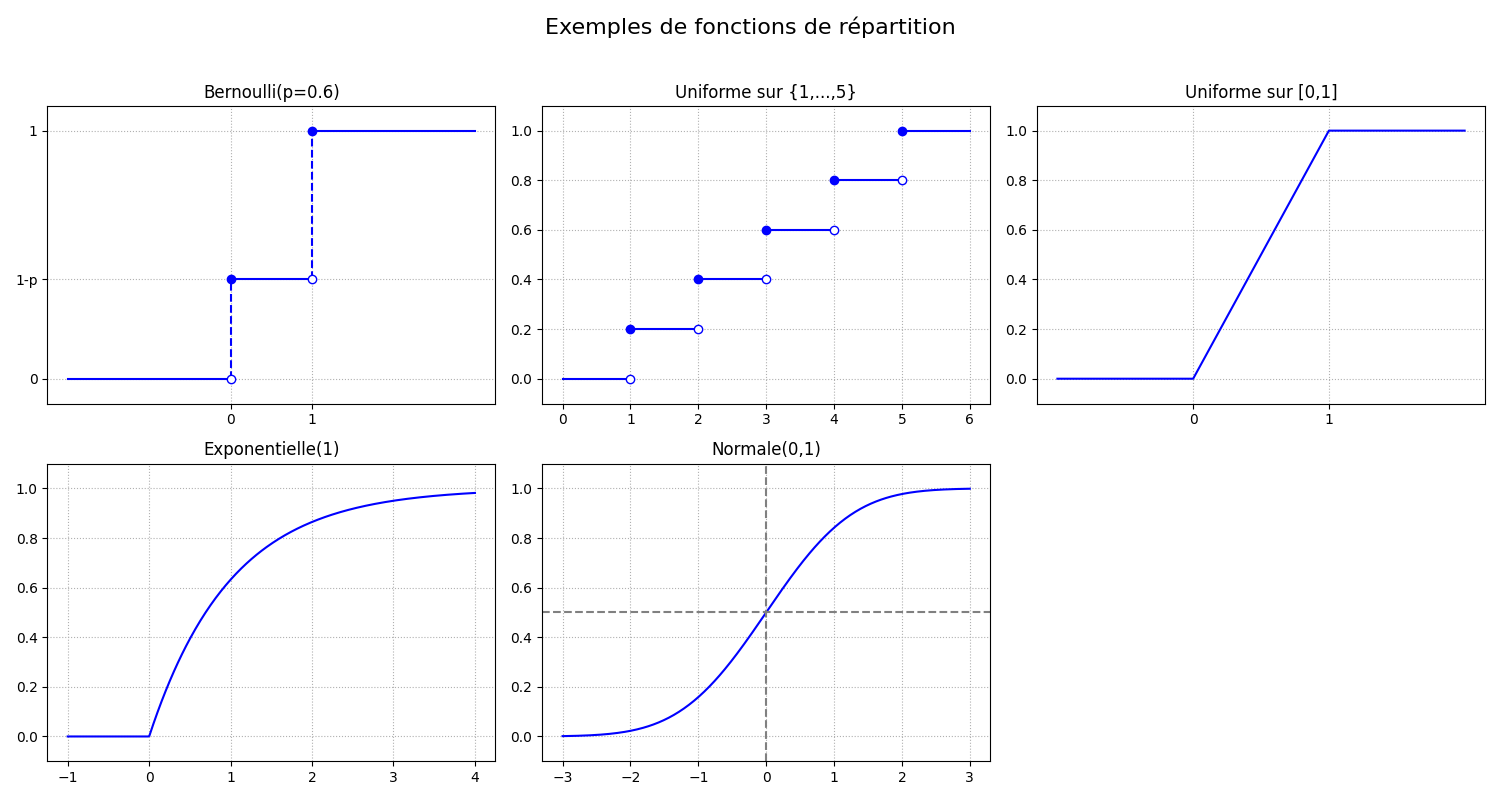
\includegraphics[width=\textwidth]{cdf_examples.png}
    \caption{Exemples de fonctions de répartition.}
    \label{fig:cdf_examples}
\end{figure}
\end{example}
Plus généralement, si la loi de $X$ admet une densité $f$, alors sa fonction de répartition est donnée par
\[
F_X(x) = \int_{-\infty}^x f(t) dt.
\]
\begin{theorem}
Notons $\mathcal{M}_1(\mathbb{R})$ l'ensemble des mesures de probabilité sur $(\mathbb{R}, \mathcal{B}(\mathbb{R}))$ et $\mathfrak{R}$ l'ensemble des fonctions qui satisfont les trois propriétés d'une fonction de répartition. L'application $\mu \mapsto F_\mu$, où $F_\mu(x) = \mu((-\infty, x])$, est une bijection de $\mathcal{M}_1(\mathbb{R})$ dans $\mathfrak{R}$.
\end{theorem}
Il s'agit d'un résultat difficile, qui permet notamment de construire des mesures de probabilités singulières sur $(\mathbb{R}, \mathcal{B}(\mathbb{R}))$.
\begin{example}[Construction d'une loi singulière]
On peut construire une suite de fonctions de répartition $(F_n)$ sur $[0,1]$ qui converge uniformément vers une fonction continue $F_\infty$, la fonction de Cantor. Cette fonction $F_\infty$ est une fonction de répartition, mais la mesure de probabilité associée $\mu$ est singulière par rapport à la mesure de Lebesgue $\lambda$. Elle ne possède pas d'atomes ($\mu(\{x\})=0$ pour tout $x$) et est concentrée sur un ensemble de mesure de Lebesgue nulle (l'ensemble de Cantor).

\begin{figure}[H]
    \centering
    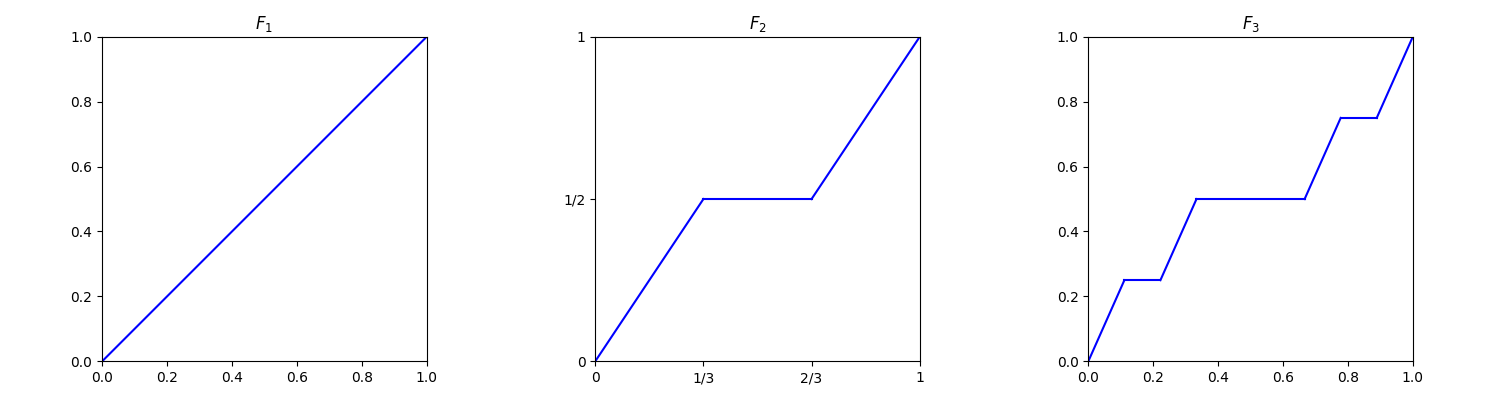
\includegraphics[width=0.8\textwidth]{cantor_construction.png}
    \caption{Premières étapes de la construction de la fonction de Cantor.}
    \label{fig:cantor}
\end{figure}
\end{example}
\section{Convergence en loi et fonctions de répartition}
Comme la convergence en loi porte sur les lois de v.a., elle doit pouvoir s'exprimer via les fonctions de répartition.
\begin{theorem}
Soit $(X_n)_{n \in \mathbb{N}}$ une suite de variables aléatoires réelles et $X$ une autre v.a. réelle. Notons $(F_n)_{n \in \mathbb{N}}$ et $F$ leurs fonctions de répartition associées. Les affirmations suivantes sont équivalentes :
\begin{enumerate}
    \item[i)] La suite $(X_n)$ converge en loi vers $X$ ($X_n \xrightarrow{\mathcal{L}} X$).
    \item[ii)] En tout point $x \in \mathbb{R}$ où $F$ est continue, la suite $(F_n(x))$ converge vers $F(x)$, i.e. $\lim_{n \to \infty} F_n(x) = F(x)$.
\end{enumerate}
\end{theorem}
\begin{proof}
$(i) \Rightarrow (ii)$: Soit $x_0$ un point où $F$ est continue. Il s'agit de montrer que $\lim_{n \to \infty} F_n(x_0) = F(x_0)$.
Pour tout $\epsilon > 0$, on peut construire deux fonctions continues bornées $f_\epsilon$ et $g_\epsilon$ qui "encadrent" la fonction indicatrice $\mathbf{1}_{(-\infty, x_0]}$ de la manière suivante:
\[
f_\epsilon \le \mathbf{1}_{(-\infty, x_0]} \le g_\epsilon
\]
et telles que $\mathbb{E}[g_\epsilon(X)] - \mathbb{E}[f_\epsilon(X)]$ soit petit.
Par exemple, posons $f_\epsilon$ égale à 1 sur $(-\infty, x_0-\epsilon]$, 0 sur $[x_0, \infty)$ et linéaire entre les deux.
Posons $g_\epsilon$ égale à 1 sur $(-\infty, x_0]$, 0 sur $[x_0+\epsilon, \infty)$ et linéaire entre les deux.
\begin{figure}[H]
\centering
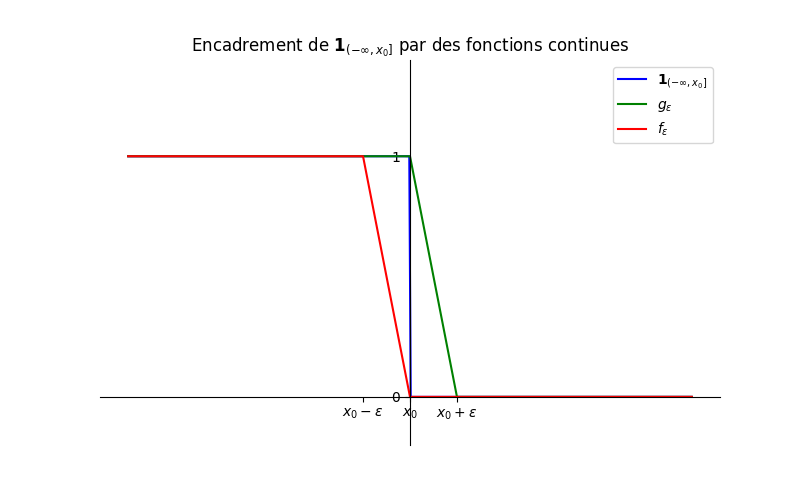
\includegraphics[width=0.6\textwidth]{sandwich_functions.png}
\caption{Fonctions $f_\epsilon$ et $g_\epsilon$ encadrant $\mathbf{1}_{(-\infty, x_0]}$.}
\label{fig:sandwich}
\end{figure}
On a $f_\epsilon(y) \le \mathbf{1}_{(-\infty, x_0]}(y) \le g_\epsilon(y)$ pour tout $y \in \mathbb{R}$. En prenant l'espérance par rapport à $X_n$:
\[
\mathbb{E}[f_\epsilon(X_n)] \le \mathbb{E}[\mathbf{1}_{(-\infty, x_0]}(X_n)] \le \mathbb{E}[g_\epsilon(X_n)]
\]
\[
\mathbb{E}[f_\epsilon(X_n)] \le F_n(x_0) \le \mathbb{E}[g_\epsilon(X_n)]
\]
Puisque $f_\epsilon$ et $g_\epsilon$ sont continues et bornées, et que $X_n \xrightarrow{\mathcal{L}} X$, on a:
\begin{align*}
    \lim_{n \to \infty} \mathbb{E}[f_\epsilon(X_n)] &= \mathbb{E}[f_\epsilon(X)] \\
    \lim_{n \to \infty} \mathbb{E}[g_\epsilon(X_n)] &= \mathbb{E}[g_\epsilon(X)]
\end{align*}
En passant à la limite dans l'inégalité, on obtient:
\[
\mathbb{E}[f_\epsilon(X)] \le \liminf_{n \to \infty} F_n(x_0) \le \limsup_{n \to \infty} F_n(x_0) \le \mathbb{E}[g_\epsilon(X)]
\]
De plus, $\mathbb{E}[f_\epsilon(X)] \ge P(X \le x_0-\epsilon) = F(x_0-\epsilon)$ et $\mathbb{E}[g_\epsilon(X)] \le P(X \le x_0+\epsilon) = F(x_0+\epsilon)$.
Donc,
\[
F(x_0-\epsilon) \le \liminf_{n \to \infty} F_n(x_0) \le \limsup_{n \to \infty} F_n(x_0) \le F(x_0+\epsilon)
\]
Comme $x_0$ est un point de continuité de $F$, on a $\lim_{\epsilon \to 0} F(x_0-\epsilon) = \lim_{\epsilon \to 0} F(x_0+\epsilon) = F(x_0)$.
En faisant tendre $\epsilon$ vers 0, on obtient par le théorème des gendarmes:
\[
\lim_{n \to \infty} F_n(x_0) = F(x_0).
\]
$(ii) \Rightarrow (i)$: 
Supposons que $F_{X_n}(x) \to F_X(x)$ en tout point $x$ où $F_X$ est continue. Soit $f: \mathbb{R} \to \mathbb{R}$ une fonction continue et bornée. Il faut montrer que $E[f(X_n)] \to E[f(X)]$.
Soit $\epsilon > 0$. Comme $\lim_{x \to -\infty} F_X(x) = 0$ et $\lim_{x \to +\infty} F_X(x) = 1$, il existe $a < b$, points de continuité de $F_X$, tels que $F_X(a) < \epsilon$ et $F_X(b) > 1-\epsilon$ (donc $P(X>b) < \epsilon$).
On décompose l'espérance :
\[ E[f(X_n)] = \int_{x \le a} f(x) dP_{X_n} + \int_{a < x \le b} f(x) dP_{X_n} + \int_{x > b} f(x) dP_{X_n} \]
Les intégrales sur les queues sont petites. Pour $n$ assez grand, $F_{X_n}(a) \to F_X(a) < \epsilon$ et $1-F_{X_n}(b) \to 1-F_X(b) < \epsilon$.
\begin{align*}
    \left| \int_{x \le a} f(x) dP_{X_n} \right| &\le \|f\|_\infty P(X_n \le a) = \|f\|_\infty F_{X_n}(a) \xrightarrow{n \to \infty} \|f\|_\infty F_X(a) \le \epsilon \|f\|_\infty \\
    \left| \int_{x > b} f(x) dP_{X_n} \right| &\le \|f\|_\infty P(X_n > b) = \|f\|_\infty (1-F_{X_n}(b)) \xrightarrow{n \to \infty} \|f\|_\infty (1-F_X(b)) \le \epsilon \|f\|_\infty
\end{align*}
Sur l'intervalle $[a,b]$, $f$ est uniformément continue. On peut l'approcher par une fonction en escalier. Soit une subdivision $a=x_0 < x_1 < \dots < x_k = b$ par des points de continuité de $F_X$. Définissons la fonction en escalier $f_k^+$ par :
\[ f_k^+(x) = \sum_{l=1}^k \mathbf{1}_{]x_{l-1}, x_l]}(x) \sup_{t \in [x_{l-1}, x_l]} f(t) \]
Alors $f(x) \le f_k^+(x)$ sur $]a,b]$. On a
\[ \int_{a < x \le b} f(x) dP_{X_n} \le \int_{a < x \le b} f_k^+(x) dP_{X_n} = \sum_{l=1}^k \left( \sup_{t \in [x_{l-1}, x_l]} f(t) \right) (F_{X_n}(x_l) - F_{X_n}(x_{l-1})) \]
En passant à la limite pour $n \to \infty$, comme les $x_l$ sont des points de continuité :
\[ \limsup_{n \to \infty} \int_{a < x \le b} f(x) dP_{X_n} \le \sum_{l=1}^k \left( \sup_{t \in [x_{l-1}, x_l]} f(t) \right) (F_{X}(x_l) - F_{X}(x_{l-1})) = E[f_k^+(X)\mathbf{1}_{]a,b]}] \]
Par continuité uniforme de $f$ sur $[a,b]$, quand le pas de la subdivision tend vers 0 ($k \to \infty$), $f_k^+(x) \to f(x)$. Par convergence dominée (car $|f_k^+| \le \|f\|_\infty$), on a $E[f_k^+(X)\mathbf{1}_{]a,b]}] \to E[f(X)\mathbf{1}_{]a,b]}]$.
En combinant les bornes sur les queues et sur l'intervalle central, on obtient pour $\epsilon$ arbitrairement petit et $n$ et $k$ assez grands :
\[ \limsup_{n \to \infty} E[f(X_n)] \le E[f(X)] \]
Un raisonnement similaire avec une fonction en escalier minorante $f_k^-$ montre que :
\[ \liminf_{n \to \infty} E[f(X_n)] \ge E[f(X)] \]
On en conclut que $\lim_{n \to \infty} E[f(X_n)] = E[f(X)]$.
\end{proof}
